
\chapter{Literature review}

\section{Hydrogen impurity enrichment}
'Hydrogen impurity enrichment' is a term for any technique which involves increasing the 
concentration of impurities within a hydrogen sample by means of removing the hydrogen matrix gas. 
There are two previous reports of impurity enrichment being used as a technique for hydrogen impurity 
analysis. 
The first report by Papadis et al at Argonne National Laboratory used a Pd/Cu \cite{Ahmed2010}
coated Pd/Ag membrane for non-sulphur containing hydrogen samples and a Pd/Au coated Pd/Ag membrane for sulphur 
containing hydrogen samples to enrich impurities in a 50 bar sample. 
The analyte gas used contained 
N\textsubscript{2}, CH\textsubscript{4} and CO\textsubscript{2} at 100 \textmu mol/mol and an additional 
 2 \textmu mol/mol of H\textsubscript{2}S during sulphur tests sulphur. 
The enrichment was calculated by using measured values of temperature and pressure along with the 
non-ideal gas law, this was represented through a 'calculated enrichment factor' as shown in equations \ref{eq:1}
and \ref{eq:2}. 

\begin{equation} \label{eq:1}
    % \frac{(\frac{P_{1,a} V_1)}{Z_{1,a} RT_{1,a}})}
    CEF_{NI} = \frac{\frac{P_{1,a} V_1}{Z_{1,a}RT_{1,a}}\frac{P_{2,a} V_2}{Z_{2,a}RT_{2,a}}-\frac{P_{1,b} V_1}{Z_{1,b}RT_{1,b}}}{\frac{P_{2,b} V_2}{Z_{2,b}RT_{2,b}}}
\end{equation}

\begin{equation}\label{eq:2}
    y_{i,a} = \frac{y_{i,b}}{CEF}
\end{equation}
The set-up was able to reach enrichment factors of around 32 for non-sulphur tests and 15 
for sulphur tests. The non-sulphur tests closely matched with the actual component concentrations, 
however in the second set of tests there was some loss of sulphur observed, most likely due to the 
formation of palladium sulphide on the surface of the membrane, or through wall catalysed reactions. 

A similar experiment was performed by National Physical Laboratory with the aim of decreasing the uncertainty 
of using such a device. \cite{Murugan2014} The non-ideal gas law method used in the previous paper \cite{Ahmed2010} 
was compared to a novel tracer enrichment method developed by NPL. \cite{Murugan2014} 
The tracer enrichment method involves spiking the hydrogen sample with a known quantity of krypton prior to 
enrichment. The enrichment factor is then calculated using the change in concentration of the krypton as 
shown in equation \ref{eq:3}.

\begin{equation} \label{eq:3}
    CEF_{Tracer} = \frac{y_{kr_b}}{y_{Kr_b}} = \frac{1}{y_{Kr_a}} \frac{A_{Kr_b}}{A_{Kr_a}} y_{Kr_{st}}
\end{equation}

The set-up was similar to the one used by Papadias et al \cite{Ahmed2010} and was used to enrich a 50 bar 10L hydrogen sample 
containing 1.5-2 \textmu mol/mol of CO, Kr, CH\textsubscript{4} and N\textsubscript{2}. Use of the tracer enrichment 
method reduced the associated uncertainty from 2.6\% to 1\%. 
Two tests were performed, with the second test resulting in membrane failure. 

When operating the hydrogen impurity enrichment device it was found that both methods should be used to 
calculate the CEF.\cite{Murugan2014}\cite{Murugan2015} While the tracer enrichment method has a lower uncertainty 
due to it being dependant on fewer variables, it is impossible to tell if a leak has occurred in the device 
due to the covariance 
phenomena. \cite{Murugan2014} Leaks in the enrichment device could occur due to thermal expansion of components due to heating 
to the required operating temperature or cracks forming in the membrane. The stability of membranes used in 
such a device will be discussed in the following section. During a leak it will be expected that the ratio of 
krypton, along with other impurities which are not naturally present in air, will remain constant, resulting 
in no change in the CEF. A leak will allow oxygen and nitrogen to enter the system and throw off the 
measurement of these two impurities. While the tracer enrichment method could still be used to calculate 
the amount fraction of other impurities, the non-ideal gas law method would have to be used to provide an 
accurate measurement for Oxygen and Nitrogen.

A device similar to the HIED is the Hydrogen Elimination Mass Spectrometer (HEMS) designed by Power + Energy USA. \cite{Bossard} 
The principle behind the HEMS is the same as the HIED, where a palladium membrane is used to selectively 
remove the hydrogen matrix gas and thus concentrate the impurities within the hydrogen sample. 
The output is directly fed into a mass spectrometer which allows in-situ measurements to be performed. 
The limit of detection specified by the manufacturer claims to be in the range of pmol/mol however there is 
no published information regarding the accuracy or uncertainty associated with the device. 
As of 2016 the device was discontinued by the manufacturer.

\subsection{Criteria for a hydrogen impurity enrichment material}
In order for a membrane to be suitable for hydrogen impurity enrichment material it must be able to 
increase the concentration of low-level impurities in a hydrogen sample. 
Although all past examples of hydrogen impurity enrichment have used dense membranes with an infinite 
selectivity towards hydrogen, it is theoretically possible to use a membrane which has a lower selectivity 
to perform enrichment. This would have the advantage of allowing membranes with faster flux to be used, 
greatly reducing the amount of time required for an enrichment run, while allowing cheaper materials to be 
used in place of the palladium membranes used in past studies. In order to perform this calculation, 
the following must be known:
\begin{itemize}
\item Selectivity of the membrane must be known to a high accuracy
\item Total number of moles leaving the system
\item Concentration of enriched impurities
\end{itemize}

Since the selectivity shows the ratio of substances passing through the membrane 
(i.e. H\textsubscript{2}/N\textsubscript{2} selectivity of 2 represents 2 moles of hydrogen for every 1 mole 
of nitrogen passing through 
the membrane) if both quantities are known the number of moles of impurity leaving the system through 
permeation could be easily estimated.

\begin{equation}
    n_{i_{exit}} = n_{exit_{total}}/ \alpha^{H_2 /i}    
\end{equation}

The concentration, and therefore the number of moles of impurity on the retentate side of the membrane 
could then be analysed using suitable instrumentation. These values could then be added together and 
divided by the enrichment factor in order to give the original number of moles that would be in the vessel.

\begin{equation}
    y_i=\frac{(n_{i_{ret}}+n_{i_{exit}})/n_{tot_{ret}}}{CEF} 
\end{equation}

In practice however this may not be feasible due to the low concentrations of impurities expected to be 
present in these hydrogen samples. In order for an enrichment calculation to work there must be an analysable 
concentration of impurity remaining in order to back calculate. Since the level of expected impurities in a 
hydrogen sample is so low, and the selectivity of many membranes also low, there is a high risk of either all 
impurities simply leaving the sample during the enrichment run, or only achieving a lower enrichment factor. 
Take the example of enriching a sample containing 0.2 \textmu mol/mol of CO by 100 in order to analyse its 
composition on 
a GC-MS. If the sample is a standard 10L cylinder containing 100 bar a H\textsubscript{2}/CO selectivity of 
\textasciitilde 4950000 is required to simply prevent all of the CO leaving the enrichment device, which is 
effectively the 
same as the selectivity’s seen in dense metal membranes. However, for the same sample containing 0.3 \textmu mol/mol 
of 
Helium a H\textsubscript{2}/He selectivity of 330 is the minimum required which is more feasible. However, both these values 
are the exact values required by the standard, in reality they would be much lower. The highest reported 
selectivity of a non-infinitely selective membrane was Liquid crystalline polyester which had a 
H\textsubscript{2}/N\textsubscript{2} 
selectivity of  2632 \cite{Weinkauf1992} which indicates that this method may be suitable for enriching some of the higher 
concentration impurities in hydrogen samples, it is not a solution for lower concentration. 
It is also unlikely that the selectivity of a membrane material will stay constant throughout its lifespan. 
Any drift in selectivity would throw off the calculation and either require regular changing of the membrane, 
driving up cost, or regular calibration to recalculate the selectivity of the membrane at a given time, which 
would be time consuming. It is however likely that infinitely selective membranes are the only feasible 
enrichment material due to their ability to enrich every impurity in hydrogen, whereas non-infinitely 
selective membranes may be applied to analysis of individual impurities, it is unlikely such a scenario 
would occur in reality which makes them a non-ideal solution. 

\subsection{Other enrichment methods}
\subsubsection{Sorbent tubes}
The use of traps and sorbent tubes to pre-concentrate impurities in gases is very common in gas analysis, 
but only two hydrogen purity analysis standards have incorporated this technique to facilitate purity analysis. 
A method for concentrating the impurities in a sample of hydrogen using a zeolite- packed chromatographic 
column has been described in a paper by Hille \cite{Hille1990a}. The method involves flowing the gas sample into the column 
using a pump and cooling the column to a temperature that allows the impurities to remain trapped whilst the 
matrix gas passes through. The sample is then transferred to GC-MS for analysis. The enrichment factor for 
this method is determined by the flowrate and amount of time that the gas is sampled into the column. 
The method was validated by analysing gas mixtures of hydrogen containing 8.7 mmol/mol of silane. 
By enriching the sample, the signal- to-noise for the same measurement was increased by a factor of 2000 
indicating that levels in the range of 4 nmol/mol of silane would easily be measured using this method 
whereas the usual limit of detection (without pre-concentration) would have been 1 \textmu mol/mol

\subsubsection{Cryo-focusing}
A method for performing pre-concentration by cryo-focusing has been detailed in ASTM WK34574 
where the device is used to concentrate the impurities in a sample of hydrogen before introducing 
the gas to a GC-MS \cite{Murugan2015} The pre-concentration method involves trapping the impurities onto a glass bead trap 
at -150\textdegree C. By increasing the temperature of the trap all of the impurities apart from water 
are transferred to a separate Tenax trap which is cooled to -170\textdegree C. 
Upon heating once again the enriched sample is introduced to the analyser. 
Very high enrichment factors can be achieved using this method by flowing a high volume of the sample 
gas through the pre-concentration device to allow capture of the impurities whilst the hydrogen is removed. 
No information was provided in the standard to indicate the accuracy or limitations of this method.

\section{Review of hydrogen selective membranes}
The term membrane is used to describe a semipermeable barrier which selectively allows certain species to 
pass through it, while preventing or inhibiting the passage of others. The driving force for gas separation 
through a membrane is the pressure and component concentration gradients across the chosen material. 
In the context of hydrogen separation, the trans-membrane pressure and hydrogen concentration gradient 
across the feed and permeate, combined with the unique properties of the chosen separation material, 
will allow hydrogen to pass through the membrane, while preventing or inhibiting the transport of impurities 
which the membrane is not selective or less selective towards. A large number of materials have been studied 
for hydrogen separation. For the purpose of this review they will be split into four broad categories based 
on their material type and separation mechanism which is related to their pore structure (dense or porous); 
these categories are shown in Table \ref{tb:1} and visualized in Figure \ref{fig:1}.

The material, its structure with regards to pore size and pore size distribution, and surface chemistry, 
all contribute to the separation mechanism for removing hydrogen from its constituent gas mixture. 
The six main membrane separation mechanisms are visualised in Figure \ref{fig:1}, with (i) – (iv) showing the 
four separation mechanisms for gases in porous media, and (V)- (Vi) showing gas separation through dense media. 
For porous materials typically a combination of these mechanisms dictates the overall separation performance 
due to imperfections in the membranes structure. All dense membranes should be dictated by the solution 
diffusion mechanism and the presence of any other mechanisms are evidence of imperfections in the membrane. 

For most porous media, the separation mechanism is dominated by Poiseuille flow or Knudsen Diffusion. 
The precise separation mechanism can be determined by calculating the ratio between the mean free path of 
the gas molecules (\textlambda) and the pore radius (r) as shown in Equation \ref{eq:6} where \texteta \ is the viscosity of the gas, 
P is the pressure, T is the temperature, M\textsubscript{w} is the molecular weight of the gas, and R is the universal gas 
constant.

\begin{figure}
    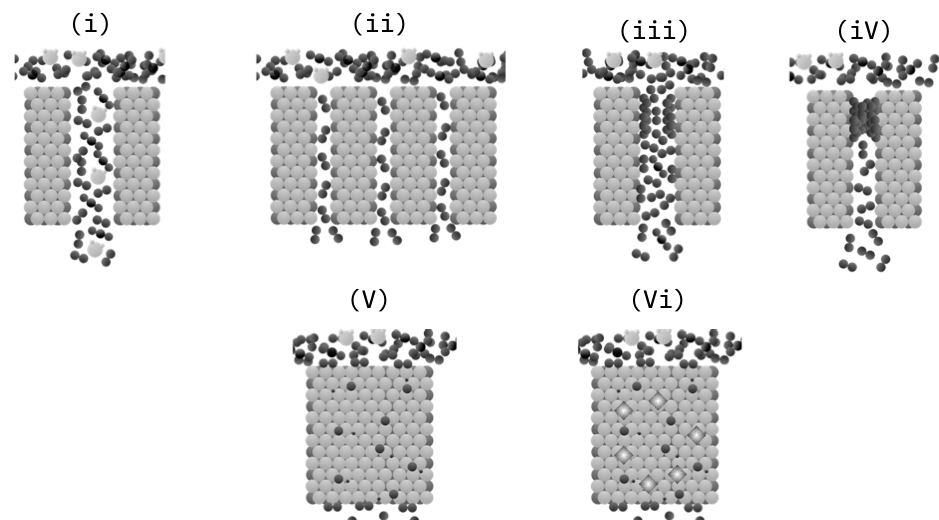
\includegraphics[width=\linewidth]{figures/septype.png}
    \caption{Illustration of the five membrane separation mechanisms (i) Poiseuille Flow/Knudsen diffusion, (ii) Molecular Sieving, (iii) Surface diffusion (iV) Capillary condensation (V) Solution diffusion (Vi) Facilitated transport}
    \label{fig:1}
  \end{figure}

\begin{equation}\label{eq:6}
    \frac{r}{\lambda} = \frac{2P}{3\eta}\sqrt{\left(\frac{2M_w}{\pi RT} \right)}
\end{equation}

This ratio determines the contribution of Knudsen and Poiseuille flow. If r/\textlambda \ > 1 it would indicate 
that the main gas transport rate limiting step is due to molecule-molecule collisions indicating that 
Poiseuille flow is the dominant transport mechanism. Likewise if r/\textlambda \ < 1 it indicates that 
molecule-wall collisions govern the rate limiting step showing that Knudsen diffusion is the dominant 
mechanism. If the transport is purely Knudsen diffusion the H\textsubscript{2}/CO\textsubscript{2} selectivity of 
the membrane will be equal to around 4.7. Since this value is relatively low, it has pushed researchers 
into fabricating membranes with smaller pore structures, and to modify their membranes to take advantage of 
specific surface interactions. Both of these developments allow researchers to surpass the selectivity 
achievable with purely Knudsen diffusion.

Molecular sieve materials can be classed as macroporous (>50nm), mesoporous (2-50nm) and microporous (<2nm) 
with microporous materials being the most relevant for hydrogen separation processes. These membranes are 
fabricated in such a way that the passageways are small enough that the entrance of molecules with large 
kinetic diameters is not possible. This results in higher permeation of smaller components in a gas mixture 
such as H2 or He while slowing, or completely preventing the passage of bulkier molecules. This mechanism, 
while effective for some gas mixtures, may not be feasible when looking to perform separation on similar 
sized gas pairs; selectivity is often hindered by competitive adsorption between the species due to the 
surface chemistry of the material. Fabrication of these membranes can also be difficult and manufacturing 
large scale membranes with a tight enough pore size distribution to ensure molecular sieving still proves 
to be a difficult task. Common microporous materials which are able to be fabricated into molecular sieving 
membranes are zeolites, metal organic frameworks, activated carbon, and amorphous silica.

Surface diffusion and capillary condensation are similar in that the surface chemistry of the pores in the 
membrane has a large effect on the separation efficiency. Surface diffusion occurs when the walls of the pore 
either intrinsically, or following modification, provides adsorption sites for the desired gas molecule. 
The gas molecule will adsorb onto the walls resulting in faster diffusion through the pore structure than 
other gases in the mixture. Similarly, capillary condensation typically follows on from surface diffusion 
and involves the gas species condensing within the pore of the membrane, either due to stronger molecule-wall 
interactions, or a smaller pore radius. The condensation of the molecule results in further selectivity 
improvements towards this component by providing an added transport barrier to other gas species. 

Gas transport in dense media is typically harder to categorise due to the unique material chemistry present 
in each material, however all dense membranes perform separation through some variation of the solution 
diffusion model. Typically, the following steps are always present in some form:
\begin{enumerate}
\item Adsorption of gas species onto the surface of the membrane 
\item Diffusion of gas species through the bulk of the membrane 
\item Desorption and diffusion of the gas species in the downstream. 
\end{enumerate}

More details will be provided on the precise features of solution diffusion in each material in the following 
sections. Facilitated transport is a sub section of solution diffusion and occurs in dense membranes which 
have a selected chemical species added into the bulk of the membrane. These materials are chosen based on the 
presence of a particular interaction with components of a gas species. These interactions are typically 
reversible reactions between the added species and the gas intended for separation and is intended to enhance 
the diffusion of the selected gas, this additive could either be fixed species (solid) or mobile (liquid). 

The most commonly reported metrics for membrane performance is the flux or permeability coefficient and 
selectivity. The flux (J) of a membrane is a measure of the amount of gas the membrane is allowing to pass 
per unit time per unit surface area and is typically used as a measure for how effective the fabricated 
membrane performs. The permeability coefficient (P) can be derived from the flux and is a quantitative 
expression which gives a specific measure of the separation properties of a material independent of 
operational and manufacturing constraints such as operating pressure and membrane thickness. 
While flux and permeability are similar and tied to each other they are both useful in their own way. 
The permeability coefficient is typically tied to the material and is useful for comparing different 
materials to each other, while the flux offers a measure on how effective the material is when fabricated 
into a membrane. 

The selectivity (\textalpha \ i/j) represents the separating ability of the membrane for a specific gas species 
(i) with respect to another gas species (j). This is common notation for porous membranes and membranes which 
are not completely selective towards one component. For membranes which are only selective towards one 
component such as dense metal and dense ceramic, the selectivity is not reported since any presence of 
another component in the exit stream is generally an indication of a manufacturing defect. 

While these values are reported for all membranes in order to allow for a direct comparison of 
performance, this is where the similarities end. The fundamental separation mechanism, manufacturing 
techniques, and unique material chemistry are often different for each material. In addition to this 
there are other important metrics for the usefulness of a membrane such as mechanical stability, lifespan, 
and chemical resistance which are more difficult to quantify. 


\subsection{Types of hydrogen separation membrane}
\begin{table}[htbp]
	\centering
	\caption{Types of hydrogen separation membrane}
	\resizebox{\textwidth}{!}{\begin{tabular}{LLLLLL}
		\hline
		\textbf{Material} & \textbf{Separation mechanism} & \textbf{Mechanical stability} & \textbf{Chemical Stability} & \textbf{Operating temperature} & \textbf{Selectivity} \\ \hline
		Polymer (Dense) & Solution diffusion, Facilitated transport &  Susceptible to Compaction 6 and Swelling 7
        & A & A & A \\
		Polymer (Porous) & Knudsen diffusion, Molecular sieving, Surface diffusion, Capillary condensation, Poiseuille flow  & Susceptible to Compaction 6 and Swelling 7 & Low chemical stability, Degrades under H\textsubscript{2}S, HCl, CO\textsubscript{2}, SO\textsubscript{x} 8
         & <100\textsuperscript{O}C & 2.5 9 –960 10
         (H2/N2 selectivity)         \\
		Nano-porous & Knudsen diffusion, Poiseuille flow, Capillary condensation, Surface diffusion, Molecular sieving & Brittle & Good 11 & Ambient -500\textdegree C & 2.4 12 -  1000 13
        (H2/N2 selectivity)
         \\
        Dense Metal & Solution Diffusion & Phase transition 14
        Dependant on support 14
        Surface segregation14
        & Negative interaction with CO, CH\textsubscript{4}, and H\textsubscript{2}O. Reacts with H\textsubscript{2}S and SO\textsubscript{x} 14 & 300-600 15 &  $\infty$ \\ 
        Dense Ceramic & Solution Diffusion & Brittle
        Difficult to seal due to high operating temperature
         & Degrades under CO\textsubscript{2} 16 & 500-1000 16
         & $\infty$ \\ \hline
	\end{tabular}}\label{tb:1}
\end{table}

\subsubsection{Micro-Porous materials}
Micro-porous materials are a class of materials generally used to refer to inorganic 
materials which possess small pores on a micrometre scale. Due to wide ranging scale of the 
term and the large volume of literature available on the following topics this section will 
aim to give a brief overview of each technology and identification of new trends in the field.
For more information on each topic the following reviews can be referred to for zeolites 
11,17–22, micro porous silica 11,17,23, carbon molecular sieve membranes 11,17,24–27, and 
Metal Organic Frameworks (MOFs).28–35 A direct comparison of recently reported micro-porous 
material membranes can be found in \textbf{'APPENDIX TABLE'}.

\paragraph{Zeolites} are a class of crystalline inorganic framework based on aluminosilicate minerals, 
and are the most widely resmearched class of micro-porous material. Zeolites are a popular 
choice for separation material due to their good thermal and chemical stability, and have 
been successfully applied to a number of fields including being fabricated into membranes 
for a range of gas separation applications.11 Zeolites can either occur naturally, or 
synthesised both at laboratory or industrial scale. 36  There are around 45 naturally 
occurring zeolites and an additional 232 synthetic zeolites, each given a three letter 
designation when approved by the International Zeolite Association Structure Commission. 37

The porosity and pore structure of a zeolite membrane is tightly tied to the chosen zeolite38. 
The final separation efficiency of a zeolite membrane is typically dictated by the method 
used to prepare it. In practice a zeolite membrane will have some degree of polycrystallinity 22,39 
due to the nature of the crystallisation based synthesis methods used. 
This will cause the formation of grain boundaries on the membrane, interrupting the 
homogeneity, and therefore the pore structure of the zeolite layer. One of the main 
challenges in scaling up production of zeolite membranes revolves around minimising or 
predicting the effects of this phenomena. 

Depending on the zeolite chosen, molecular sieving is possible assuming a continuous layer is 
deposited. In particular LTA 40 and MFI 41 show the greatest potential for hydrogen separation, 
showing separation performance surpassing that of Knudsen diffusion 42,43 and the ability to 
operate at temperatures ranging from ambient 42 to 500 \textdegree C 43. Current research 
trends still show that synthesis is the biggest target for researchers. 39 Some researchers 
have looked to 
the support as a place to improve the synthesis of zeolite membranes by incorporating 
3-aminopropyltriethoxysilan, PDA or ZnO into the inorganic support in order to improve 
adhesion, reduce the coarseness of the support, and enable the fabrication of thinner, 
more homogenous layers. The addition of these materials onto the support can also allow the 
support directing agent, and in some cases the seeding step altogether, too be bypassed. 
Minimising the use of support directing agent in the manufacture is advantageous since 
support directing agents typically slow the growth of zeolite, drive up cost and must be 
removed after synthesis, which could damage the membrane. 36 The addition of these materials 
on the support allows for covalent linkers to form between the support and zeolite, which 
assists the migration of zeolite particles during hydrothermal synthesis. 44

While zeolites have been researched for a number of decades and there have been many 
developments in microstructure tailoring, fabrication procedures, and thin film deposition, 
adoption of zeolite membranes have still been limited. This can mainly be attributed to the 
fact that the highest performing, and therefore most attractive, zeolite types are still 
difficult to synthesise on a large scale. While there has been some progress with the 
synthesis of sub-micron layers suitable for other separations, there is little published 
evidence that these layers are usable for the light gas separation required for large scale 
hydrogen production. Until this hurdle can be overcome it is unlikely that the technology 
can be used commercially. 45 Currently zeolite membranes have only been used commercially 
for liquid separation and with current research trends turning away from zeolites to newer 
classes of materials, their application may be limited to this area. This loss of interest 
is likely due to the lack of reproducibility to meet the standards required for industrial 
applications, therefore driving down the interest. 

\paragraph{Micro porous silica} membranes are amorphous structures which generally display tight pore 
size distributions and can be more easily fabricated into thin films than zeolites. They 
are an attractive option for large scale gas separations due to the low cost of the precursor 
materials required to fabricate the membrane. Silica membranes are typically composed of a 
three-layer structure; the membrane layer which is generally an ultra-microporous layer of 
the silica, an intermediary porous layer typically of the same silica material, and an 
inorganic porous support typically ceramic. Silica membranes are formed from networks of 
micropores typically on the scale of 0.5nm in diameter, giving them the potential to achieve 
molecular sieving separation similar to, or surpassing that of zeolites. 

From the membranes mentioned in Table 4 it is clear that silica membranes are an attractive 
option due to their extremely efficient separation characteristics. Silica membranes are able 
to achieve massive selectivity towards hydrogen, with some membranes reporting a H\textsubscript{2}/CO\textsubscript{2} 
selectivity greater than 1,000 46 with permeabilities on the scale of 10\textsuperscript{-7} mol/(m\textsuperscript{2} s pa) 
47. Many of the reported membranes are on the scale of \textless 100nm 47–49 which, if scalable, 
would result in a massive cost reduction when compared to other membrane types which require 
thicker layers to achieve usable separation performance. 

Silica membranes have been successfully applied on a lab scale however they experience 
stability issues, which must be overcome before they can be applied to a specific application. 
Silica membranes are highly unstable at high temperature and are easily attacked by moisture 
which causes the condensation of silanol groups in the silica layer, destroying the structured 
pores in the material. 50 The most common strategy to try and overcome this is to induce 
hydrophobicity to the membrane by incorporating a metal or metal oxide into the matrix.  
The thought process behind this is that the oxygen will form preferential bonds with the 
metal instead of the silanol group therefore maintaining pore structure. While this method 
seems promising, and may improve performance, it is unclear from literature if any long term 
stability studies have been performed to test if this is a lasting improvement. The most 
common metal dopants for this purpose are cobalt 47,51, iron, nickel and niobium 46,52. 
Additionally hydrophobicity could be induced by replacing some of the silanol groups on the 
surface of the membrane with carbon groups as shown by Lee 13,48,53. 

\paragraph{Carbon based membranes} come in many forms with the most common being carbon 
molecular sieve membranes but can also be extended to graphene. 

In theory any carbon containing compound could be used to manufacture a carbon molecular 
sieve membrane, however synthetic polymers are typically preferred due to their ability to 
be easily processed into homogeneous films which are essential for forming a homogenous 
carbon film.26  The precursor material should also show good thermal stability and not melt 
or soften during the pyrolysis step, again to ensure a homogenous carbon layer is formed. 25

Carbon molecular sieve membranes are typically stable in most environments, however suffer 
in the presence of oxygen and water due to the materials readiness to oxidation. 27 Due to 
this carbon molecular sieve membranes typically see large permeability reduction when exposed 
to small levels of these impurities. 27

Although zeolites and MOF’s often show higher separation performance than carbon molecular 
sieves, their high fabrication cost limits their use to processes with high margins. 
Carbon molecular sieve membranes can overcome the limitations of other porous materials 
while theoretically maintaining a cost similar to that of polymer membrane systems. 24 
While the theoretical cost of producing carbon molecular sieve membranes is low, its current 
cost is high due to the popularity of polyimide as a precursor. Since many carbon molecular 
sieve membranes are manufactured from polymers which are already used in the fabrication of 
polymer membranes it is unlikely that choosing to make them into carbon molecular sieve 
membranes will be an economical option. In order for the technology to flourish in industry 
alternative precursors must be researched and commercialised. 

Graphene and its variations have also seen some success when applied to hydrogen separation. 
Graphene is the term used to refer to a single layer of sp2 hybridised carbon. Due to the 
ultrathin nature of graphene, along with its strong mechanical and chemical stability, it 
makes an extremely attractive choice for a membrane material. 54 A dense layer of graphene 
is completely impermeable to gases and therefore further modification is required in order 
to bring about any separation behaviour. 55 Gas separation behaviour in graphene membranes 
is normally induced through the introduction of defects, this can either be defects which 
are present from the manufacturing process as shown in the papers published by Kim 56 and Zhu 57, 
or through post treatment of a dense graphene layer commonly through methods such as 
ultraviolet induced oxidative etching or oxygen plasma etching as performed by Celebi et al. 
58 While these techniques have the potential for producing high performing membranes, 
synthesising pristine, large area, graphene on a large scale still remains a problem and 
even small areas are costly to produce. 55  The defect-based nature of graphene based 
membranes also makes their commercial use questionably as there is little evidence that 
many of the reported membranes have repeatable performance characteristics. It may be that 
many of the reports are statistical anomalies and the technology simply will not show the 
repeatability to provide a commercial solution for light gas separations.

\paragraph{Metal-organic frameworks} are a new class of porous material. Similar to zeolites 
the material displays an intrinsic porosity, however unlike zeolites MOF’s have the additional 
advantage that their structures are highly tuneable past the porosity achieved intrinsically 
through the crystalline structure. 28 MOFs are compounds which consist of a metal ion, or 
clusters of metal ions, coordinated to organic ligands to form one, two- or three-dimensional 
structures. The study of MOFs is similar to zeolites and due to the field’s infancy, takes 
much inspiration from the zeolite field. For this reason, the field was able to develop 
quickly on the back of already established methods. MOF’s are unique in that their structures 
are more flexible than that of zeolites which would allow their separation properties to 
change with the operating conditions including temperature, humidity and light. 

Due to the resurgence of the hydrogen economy in recent years there have been many reports of 
the application of MOF membranes for the selective permeation of hydrogen. Due to the tuneable 
nature of MOF’s, the field comprises of two main concepts when developing a new membranes, 
taking advantage of the size and shape selectivity of the chosen MOF to enhance molecular 
sieving behaviour, and optimising the preferential adsorption properties of the MOF to enable 
improved separation properties through capillary condensation and surface diffusion. 

In particular ‘zeolitic immobilized frameworks’ or ZIF’s have seen particular interest in the 
hydrogen separation field. ZIFs are a class of metal organic framework which topologically 
have the same crystalline structure as zeolites, while still allowing for the fine-tuned 
separation properties seen in other MOFs. ZIF’s are often applied to hydrogen separation 
applications due to its high stability and affinity towards adsorption of hydrogen. ZIF-8, 
which appears to be the most popular choice for fabrication of MOF membranes for hydrogen 
separations in recent years, has a pore size of around 3.4Å and has been successfully applied 
to hydrogen separations, however results vary a lot with reported permeability values for the 
MOF ranging from as high as 2.1x10 \textsuperscript{-5} mol/(m\textsuperscript{2} s pa) 59 
to as slow as 6.59x10\textsuperscript{-8} mol/(m\textsuperscript{2} s pa) 60 depending on the 
operating conditions. This variability is also seen in the selectivity with reported 
H\textsubscript{2}/CO\textsubscript{2} 
selectivity’s ranging from 4 60 to 25 61, showing, that similar to zeolites, the field still 
has some consistency issues with the fabrication step which must be resolved before scaling 
up. 

MOF’s have seen intense research focus in the past 10 years however, similar to zeolites, 
they have yet to be applied to any industrial application.  The issue appears to be related 
to the fact that despite there being a large number of MOF’s, there is only a small subsection 
which are stable at ambient conditions. Most MOF’s are susceptible to attack by humidity, 
decompose under heat, and are difficult to functionalise as a membrane.  62 Despite the high 
separation performances which have been reported in literature, this technology may be 
destined for the same fate as zeolites where the lack of tight reproducibility in their 
manufacturing will hinder their commercial application. 

\subsubsection{Polymers}
Organic polymers have been a mainstay in the membrane research area since their original 
commercialization by Dupont in the mid-1970’s 63  and have become common place in many 
industrial and commercial processes. Polymeric membranes for purification of hydrogen has 
been a popular target for the technology and is one of the few membrane technologies which 
has seen widespread commercialisation by a number of companies including Air Medal Products, 
64 BOC 65 and Linde Group 66.

Dense polymer membranes use the difference between solubility and diffusivity of different 
gases within the polymer as the solution diffusion rate limiting step. Generally speaking, 
polymer membranes for gas separation are regarded as either hydrogen selective (H\textsubscript{2}/CO\textsubscript{2} 
selectivity > 1) or CO\textsubscript{2} selective (H\textsubscript{2}/CO\textsubscript{2} 
selectivity < 1). Both types of membranes can be used for hydrogen separation with the 
only difference being whether the hydrogen is recovered from the permeate or retentate side.  
‘Glassy’ polymeric materials such as poly-sulfone tend to be hydrogen selective due to their 
rigid structure and small free volume. 11 ‘Rubbery’ polymeric materials such as 
poly(dimethylsiloxane) tend to be CO\textsubscript{2} selective. 11

Polymer membranes are typically produced through polymer phase separation whereby a chosen 
polymer material is mixed with a solvent where it is subsequently separated through either 
non-solvent induced phase separation, or temperature induced phase separation. 
The result is a membrane composed of a dense and thin skin layer ranging between 0.1-0.5 
$\mu$m 11 which performs the separation, and a microporous support structure composed of the 
same material providing mechanical strength for the membrane. 

Polymer membranes are popular within industrial separation processes due to their low 
manufacturing cost, ability to operate at low temperatures (around 25\textdegree C), and 
ease of scaling. There are however several issues with polymer membranes which limit their 
applications. The main limitation of polymer membranes is their low stability in chemically 
aggressive environments. In particular polymeric membranes are susceptible to CO\textsubscript{2} 
degradation and are highly susceptible to fouling by sulphur containing compounds. With these 
two impurities being commonly found in hydrogen streams this poses an obvious issue with 
regards to a system using polymer membranes. The normal solution to this is simply to remove 
these impurities prior to the membrane separation step. However, polymer membranes are also 
susceptible to mechanical problems such as swelling, compaction, 6 and degradation at higher 
temperatures which can limit their lifespan. \textbf{APPENDIX TABLE} shows a direct comparison 
of a sample of literature reporting the performance of polymer membranes.

\subsubsection{Dense metallic}
Metallic membranes are comprised of dense metal or alloy sheets which allow the permeation 
of hydrogen through its constituent electrons and protons. While this is the same separation 
mechanism seen in dense polymer membranes the hydrogen selectivity is typically a lot higher 
in these systems since molecules which are not hydrogen are unable to dissociate and permeate 
through the membrane surface, giving a theoretically infinite selectivity towards hydrogen. 
The minimum requirement for a dense metal membrane for hydrogen separation is the ability to 
dissociate and permeate hydrogen. There are a number of metals which have shown varying 
degrees of suitability for hydrogen separation and these are shown in Table \ref{tb:2}.



\begin{table}[htbp]
    \centering
    \caption{Metals which show the ability for hydrogen permeation 11}
    \resizebox{\textwidth}{!}{\begin{tabular}{@{}ccccc@{}}
    \toprule
    Structure            & Metal & \begin{tabular}[c]{@{}c@{}}Activation energy for \\ \\ hydrogen permeation (kJ/mol)\end{tabular} & \begin{tabular}[c]{@{}c@{}}Heat of hydride \\ \\ formation (kJ/mol)\end{tabular} & \begin{tabular}[c]{@{}c@{}}Hydrogen permeability at \\ \\ 500\textdegree C (mol/ m s $pa^{1/2}$)\end{tabular} \\ \midrule
    \multirow{4}{*}{fcc} & Ni                         & 40.0                                                                                             & -6                                                                               & $7.8*10^{-11}$                                                                                      \\
                         & Cu                         & 38.9                                                                                             & -                                                                                & $4.9*10^{-12}$                                                                                      \\
                         & Pd                         & 24.0                                                                                             & 20                                                                               & $1.9*10^{-8}$                                                                                       \\
                         & Pt                         & 24.7                                                                                             & 26                                                                               & $2.0*10^{-12}$                                                                                      \\
    \multirow{4}{*}{bcc} & V                          & 5.6                                                                                              & -54                                                                              & $1.9*10^{-7}$                                                                                       \\
                         & Fe                         & 44.8                                                                                             & 14                                                                               & $1.8*10^{-10}$                                                                                      \\
                         & Nb                         & 10.2                                                                                             & -60                                                                              & $1.6*10^{-6}$                                                                                       \\
                         & Ta                         & 14.5                                                                                             & -78                                                                              & $1.3*10^{-7}$                                                                                       \\ \bottomrule
    \end{tabular}}\label{tb:2}
    \end{table}

The flux of a dense metal membrane is given by Eqn \ref{eq:7} and is a function of the metals 
permeability to hydrogen, the concentration and pressure gradient across the membrane, and 
the thickness of the dense layer. 

\begin{equation}\label{eq:7}
    J=\frac{\phi}{l} (P_{H,ret}^{0.5} - P_{H,perm}^{0.5})
\end{equation}

From the metals shown in Table \ref{tb:2} palladium and its alloys are by far the most 
popular choice due to a combination of high hydrogen permeability, favourable catalytic 
activity towards hydrogen dissociation and re-association, and aversion towards hydride 
formation compared to other metals. 11,67,68  

For other metals there is often a trade-off, V, Nb and Ta exhibit higher permeability than 
palladium but are limited by their low catalytic activity for hydrogen dissociation and 
typically must be combined with another metal to compensate for this. A common strategy is 
to deposit palladium particles on both sides of membranes made from these metals to provide 
this catalytic activity. Embrittlement of pure metal membranes is also an issue, even for 
metals with a high heat of hydride formation. Embrittlement is a side effect of hydrogen 
passing through the crystal lattice. During transport a H-M phase will form which has a 
higher lattice parameter than the original crystal lattice. This change in lattice parameter 
can cause stress in the overall structure of the dense membrane layer and cause the formation 
of pin holes, cracks, and eventually membrane failure. Metals with a low heat of hydride 
formation in Table \ref{tb:2} will readily embrittle within hydrogen containing atmospheres.

This section will discuss developments in both palladium and non-palladium membranes and the 
issues still surrounding the technology.

As previously mentioned palladium is typically the material of choice for dense metallic 
membranes due to its combination of high stability, permeability, and catalytic activity. 
Palladium based membranes have been successfully used to provide ultrapure hydrogen for a 
number of applications including electronics, industrial gas, and fuel cell industries for a 
number of years. The main downside to the use of palladium is its high cost of around \$25 
per gram. 69 This high cost has pushed researchers into focusing on reducing the amount of 
palladium used in the membrane in order to find a more economical solution. This is done 
either by using a traditional membrane approach, whereby the thickness of the membrane layer 
is reduced as much as possible to maximise the flux while decreasing the overall amount of 
palladium used, or by alloying palladium with a cheaper metal to reduce the amount of bulk 
palladium in the manufacturing process. 

During operation of a pure palladium membrane at temperatures lower than 300\textdegree C, 
hydrogen embrittlement can occur due to the aforementioned phase transition between 
interstitial hydrogen within palladium ($\alpha$ phase) and palladium hydride ($\beta$ phase). 
The $\beta$ phase (0.4025 nm) has a lattice parameter bigger than the $\alpha$ phase 
(0.389nm). 70  The formation of this $\alpha$ - $\beta$ phase will cause the membrane to distort, 
become brittle, and eventually results in membrane failure when a leak occurs. 71 
Aside from this pure palladium has poor chemical stability, it can be poisoned by a 
number of impurities which are commonly found in hydrogen. Some of these impurities 
simply inhibit permeation of hydrogen but do not have a permanent interaction and thus 
their effects can be mitigated by optimising the operating conditions. Others such as 
H\textsubscript{2}S and CH\textsubscript{4} are known to interact with the membrane through chemisorption and permanently 
damage the membrane through the formation of compounds with palladium, breaking the 
crystalline lattice resulting in membrane failure.  

From the impurities listed in Table 1 CO, H\textsubscript{2}O, Hydrocarbons and sulphur 
containing compounds are known to have a physisorption interaction with palladium. 
Physisorption based poisoning occurs by the impurity inducing a competitive adsorption 
with hydrogen, blocking active sites for hydrogen dissociation, and hence reducing the 
active area available for hydrogen permeation.14 The ultimate effect of this is a temporary 
flux reduction which has no long lasting damage on the membrane. Compounds such as 
H\textsubscript{2}S, and CH\textsubscript{4} have a more extreme effect on the membrane as 
adsorption leads to a reaction between palladium and the metal permanently changing the 
membrane composition and structure. The most commonly studied interaction is the interaction 
between palladium and H\textsubscript{2}S to form palladium sulphide. Palladium sulphide, while still
permeable to hydrogen, has an extremely low permeability, drastically reducing the efficiency 
of the membrane. Palladium sulphide also has a larger lattice constant than that of pure 
palladium which can lead to membrane failure by creating gaps in the crystal lattice 
resulting in pinholes. Some of these impurities, in particular those which only exhibit 
physisorption, can be mitigated by altering the operating conditions. It has been reported 
that the effects of CO and H\textsubscript{2}O poisoning can be completely eliminated by operating at 
temperatures above 300\textdegree C. Another example where this is shown is with H\textsubscript{2}S related poisoning. 
Since the reaction between palladium and H\textsubscript{2}S is exothermic, and produces hydrogen as a side 
product, it can be inhibited by increasing the H\textsubscript{2}: H\textsubscript{2}S ratio and increasing the temperature.  

A combination of cost, readily formation of phase transitions 70,71 and its low tolerance for 
common impurities found in hydrogen processes limits pure palladiums use as a hydrogen 
separation material. Many of these effects however, can be completely mitigated through 
alloying palladium with another metal. By forming an alloy with a metal which has a lattice 
parameter similar to that of the $\beta$-phase the average difference between the sizes of 
the two phases is effectively decreased and thus the hydrogen embrittlement effect can be 
effectively mitigated. The effect of impurities on palladium membranes can also be partially 
mitigated by alloying with another metal and oftentimes an increase in permeability is 
reported with certain alloy compositions. 

Both binary and ternary alloys of palladium have been reported and is a mature topic in 
literature. By far the three most popular alloying compounds with palladium are silver, 
copper and gold. The current literature landscape of palladium alloy membranes are summarised 
in \textbf{BIG METAL TABLE} and for the purpose of this review studies which looked at the impurity resistance, which 
is currently the most pressing issue in the field, were focused on. 

Silver is the most popular dopant for palladium membranes and forms a stable alloy with 
palladium at concentrations greater than 20wt \%, with the optimal composition occurring at 
23\%. On top of mitigating the effects of hydrogen embrittlement, a ~60\% increase in 
permeability is observed when compared to pure Pd membranes. Despite having enhanced 
permeation properties, PdAg is still susceptible to poisoning, in particular from sulphurous 
compounds which can form both Pd\textsubscript{4}S and Ag\textsubscript{5}Pd\textsubscript{10}S\textsubscript{5}. Several studies exposing PdAg membranes 
to sulphurous compounds have been performed and in most cases the membranes suffer a large 
decrease in flux, and are permanently damaged as shown by a permanent decrease in flux when 
sulphide is removed from the inlet. 72 It has been observed that exposure to 5 \textmu mol mol\textsuperscript{-1} H\textsubscript{2}S 
in the feed stream is enough to induce Pd\textsubscript{4}S formation 73 and therefore this composition is 
only suitable for atmospheres and applications which do not contain any sulphur. 

Copper is another widely studied binary alloy which is known to suppress hydrogen 
embrittlement. Alloying with copper also has the advantage that it reduces the cost of the 
membrane by a larger amount than most other metals and through improving the membranes 
sulphur resistance. The maximum permeability of a palladium copper membrane occurs at the 
composition Pd\textsubscript{60}Cu\textsubscript{40} and this is due to the formation of a 
bcc lattice rather than the fcc lattice commonly seen in pure palladium and most binary 
alloys. 74 Temperature cycling has been performed on this alloy composition and it has been 
found that the bcc crystalline configuration has a higher permeability than the fcc phase. 75 
This behaviour is due to the increased number of hcp adsorption sites which hydrogen has a 
slight preference for.76 Conversely the fcc structure has a higher impurity resistance 
than the bcc structure, particularly for H\textsubscript{2}S. This has been theorised to be because 
adsorption of H\textsubscript{2}S on a palladium membranes surface is largely controlled by electronic 
factors.77 There have been several studies reporting an increased resistance to sulphur 
poisoning by alloying palladium with copper. A Pd\textsubscript{80}Cu\textsubscript{20} 
membrane exposed to 20 \textmu mol $mol^{-1}$ of H\textsubscript{2}S for 90 hours results in a 
22\% drop in flux, performing much better than Pd\textsubscript{75}Ag\textsubscript{25} reported in the same paper which 
became impermeable after 65 hours of exposure in the same conditions.73 In a similar study, 
the performance of bcc and fcc alloys in response to H\textsubscript{2}S 
Pd\textsubscript{20}Cu\textsubscript{80}, Pd\textsubscript{40}Cu\textsubscript{60} and 
Pd\textsubscript{53}Cu\textsubscript{47} foils at varying temperatures was tested in 
hydrogen containing 1000 µmol $mol^{-1}$  H\textsubscript{2}S.78 It was found that when the alloys were in the 
fcc phase the reduction in flux was only round 10\%, while in the bcc phase the membrane 
loses around 99\% of its permeance. The H\textsubscript{2}S concentration required to make a 
Pd60Cu40 membrane completely impermeable was found to be around 300 µmol $mol^{-1}$ 79.

PdAu alloys see a slight increase in permeability,  up to 30\% more than pure Pd, with gold 
additions up to 20\%, after which the permeability rapidly decreases. While alloying with 
gold does not improve the permeability much compared to silver or copper, gold alloys show 
greatly improved sulphur resistance. Several studies have been performed which show that PdAu 
membranes show no permanent permeability loss after exposed to ppm levels of sulphurous 
compounds implying that permeability decline is only due to H\textsubscript{2}S adsorption. 
It has been reported that a Pd\textsubscript{92}Au\textsubscript{8} membrane exposed to 
54.8 µmol $mol^{-1}$ of H\textsubscript{2}S was able to resist reaction with H\textsubscript{2}S and its permeability was 
completely recoverable. 80. When tested higher temperatures it was also found that the 
adsorption effect of H\textsubscript{2}S was reduced which is evidence that dissociative adsorption of H2S 
on metals is exothermic. 80 In the original patent for palladium membranes by  McKinley81 
in 1964 Pd\textsubscript{60}Au\textsubscript{40} was found to be the composition which performed best under sulphur 
containing atmospheres, losing only 9.44\% of its flux compared to the 99\% and 95\% lost by 
PdAg and PdCu membranes respectively.81 However under recovery the flux increased to 120\% 
of its original value while the PdCu membrane was fully recovered under the same conditions. 
This may be evidence that the Pd\textsubscript{60}Au\textsubscript{40} membrane used is not completely stable. 81 When 
comparing the performance of PdCu and PdAu membranes under a number of gases which commonly 
result from the water gas shift reaction it was found that the PdAu resisted . 82 
It was found that from the four membranes tested, the PdAu membranes show no permeability 
loss under an atmosphere containing CO, CO\textsubscript{2} and H\textsubscript{2}O while the PdCu membranes showed 
considerable permeability loss. 82 The biggest downside to alloying with gold is that 
due to its high price in recent years alloying palladium with gold drives up the price 
higher than that of a pure palladium membrane and is one of the less economic options. 83

Other metals have been alloyed with palladium although outside of these three metals, 
studies evaluating the impurity resistance of other binary alloys are rare. The adsorption 
of CO on Pd\textsubscript{92}Y\textsubscript{8} membranes under various concentrations has been studied using TDS and XPS 
and found that CO can react with the Pd-Y allow at 623K, forming YO and solid carbon. 84  
Bryden et al studied the poisoning resistance of nanostructured palladium-iron alloys 
compared to polycrystalline membranes of the same composition. 85 They found that 
nanostructured membranes not only display higher fluxes, but also exhibit a higher 
resistance to hydrogen sulphide poisoning. When exposed to \textasciitilde 60 µmol $mol^{-1}$, 
of H\textsubscript{2}S for 2.2 hours there was no permanent reduction in flux. 
Howard et al studied the performance of PdPt\textsubscript{20} membranes under 1000 µmol $mol^{-1}$ 
H\textsubscript{2}S at temperatures between 350\textdegree C and 450 \textdegree C. 86 
The alloy had decent performance on the lower end of the temperature, only losing about 5\% 
of permanent permeability. At higher temperatures the membrane lost around 25\% of its 
permeability, much of this attributed to platinum segregation to the surface of the 
membrane.86 The impurity resistance of PdPt membranes has also been studied under common 
WGS compositions which concluded that small additions of Pt (Between 5-9\%) can decrease 
the flux decline caused by WGS mixtures from 39\% for pure Pd, to anywhere between 7\%-22\%.86
Platinum however does not appear to be as effective at mitigating the effects of WGS mixtures 
as alloying with Au which can completely mitigate the flux decline. 87 The use of Pd\textsubscript{95}Ru\textsubscript{5} 
membranes in syngas mixtures has been tested in WGS conditions and also showed good 
resistance to adsorbing compounds, losing only 6\% of their flux compared to the 
11\% lost by a pure Pd membrane under the same conditions.88

Ternary alloys are a newly emerging field which aims at utilizing the strengths of a binary 
alloy while mitigating its weaknesses with another component. Research in this area has 
mainly focused on ternary alloys based on copper, gold and silver however there are 
theoretically infinite combinations possible. Due to the large number of potential 
combinations Density Functional Theory (DFT) is often utilised as a method to screen for 
potential alloy compositions suitable for hydrogen permeability. 89 While there are many 
papers in this field relating to the theoretical modelling or ternary alloys there are a 
lot less regarding the practical impurity resistance of such alloys. A 
Pd\textsubscript{80}Au\textsubscript{10}Pt\textsubscript{10} membrane manufactured through 
magnetron sputtering was found to be completely resistant to H\textsubscript{2}S poisoning, 
recovering 100\% of its flux prior to exposure to impurity containing gas streams. 90 
However after long term testing, the purity of the permeate decreased which implies that 
pinholes had started to form on the membrane surface. 90 This is most likely due to 
segregation of the individual components, destabilising the structure. This was not 
confirmed in the papers analysis however. 90 The most in depth study of PdAgAu membranes 
under H2S was performed by Braun et al, who studied the performance of Pd, 
Pd\textsubscript{90}Ag\textsubscript{10}, Pd\textsubscript{78}Ag\textsubscript{9}Au\textsubscript{13}, 
Pd\textsubscript{75}Ag\textsubscript{16}Au\textsubscript{9}, and Pd\textsubscript{91}Au\textsubscript{9}. 
While all the tested membranes saw a permanent permeability loss under 100 µmol $mol^{-1}$ 
of H\textsubscript{2}S the Pd\textsubscript{91}Au\textsubscript{9}, Pd\textsubscript{78}Ag\textsubscript{9}Au\textsubscript{13}, 
and Pd\textsubscript{75}Ag\textsubscript{16}Au\textsubscript{9} all resisted bulk corrosion 
as proven by Energy-dispersive X-ray spectroscopy (EDS), with the Pd\textsubscript{91}Au\textsubscript{9} 
sample having the highest resistance to H\textsubscript{2}S atmospheres. 91,92 While this 
study shows that ternary alloys do offer an increase in impurity resistance over pure Pd and 
PdAg membranes, the original flux values are not provided so it is difficult to see if 
there are any inherent advantages over simply using a PdAu alloy. 91,92 The Materials 
and Chemistry group at SINTEF have performed the most extensive study into ternary 
alloys, 93,94 testing by far the widest range of alloys and using a combination  of X-ray 
Diffraction (XRD) and X-ray photoelectron spectroscopy to analyse the segregation behaviour 
of the ternary alloys. 28 Through alloying PdCu alloys with a third transition metal they 
found that the addition of 1\% of a transition metal component always resulted in an increase 
in permeability, likely due to a phenomenon where the activation energy for hydrogen 
permeation decreases with increasing fcc lattice constant. 27 In particular the addition of 
1\% Ta, 1\% Y and 14\% Ag resulted in an increase in permeability of 10, 45 and 65\% 
respectively when compared with Pd\textsubscript{73}Cu\textsubscript{27} membranes for 
Y and Ta, and Pd\textsubscript{65}Cu\textsubscript{35} membranes for Ag additions. 27 
In the follow up paper Pd\textsubscript{75}Ag\textsubscript{22}Au\textsubscript{3},
Pd\textsubscript{76}Ag\textsubscript{21}Mo\textsubscript{3} and Pd\textsubscript{69}Ag\textsubscript{27}Y\textsubscript{4} 
membranes were exposed to 20 µmol $mol^{-1}$ of H\textsubscript{2}S for 500 hours. 
The Pd\textsubscript{75}Ag\textsubscript{22}Au\textsubscript{3} membrane was the only 
membrane which showed no bulk sulphur formation, with the other two membrane compositions 
showing large levels of oxidation and segregation when analysed using XPS. 95 The 
PdAgAu composition has been further studied by Braun et al, 91 who backed up that small 
additions of Au to PdAg membranes can reduce the membranes reactivity with sulphides and 
would be suitable for application in a hydrogen impurity enrichment device. 
Tarditi et al, have done a similar study on the impurity resistance of PdCuAu membranes. 96 
While XRD and EDS of this alloy showed no formation of bulk sulphides, the XPS depth 
profile showed low, but measurable levels of sulphur showing that this composition has some 
reactivity with impurities. 96

Due to the high cost of palladium there is a particular interest to use alternative materials 
which still give the high selectivity intrinsic to dense metallic membranes, while reducing 
the cost, for example, by switching to a cheaper, non-platinum group metal. Non-palladium 
alloy membranes in the form of amorphous, or crystalline structures generally attract the 
most research interest.

Crystalline non-palladium membranes are generally based on Group IV based alloys and follow a 
similar philosophy to the previously discussed palladium membranes. Group IV metals are 
alloyed with other metals in order to improve their physical properties while maintaining the 
bcc structure essential for the material to transport hydrogen. Crystalline metals typically 
have the same advantages and disadvantages as palladium membranes. Recent research activity 
has focused mainly on studying how the size of the grain boundary affects the permeability 
of such a membrane, an area which has been mostly neglected in palladium research. This is 
likely due to the fact that many of these alloys are manufactured through cold work where the 
grain size can be more easily tailored than in the traditional electroless and sputtering 
methods used to manufacture palladium membranes. A key aspect of crystalline alloy research 
is the effect of nano-crystalline structures. Most research in this area has revolved around 
the addition of small amounts of elements to alloys based on either Zr or Hf to tailor these 
nano-crystalline structures and study their effects on permeability. Similarly to palladium 
alloys, dopants are generally chosen based on their effectiveness at suppressing hydride
formation, with Zr, Mo, Ru and Rh being popular choices. 97–101 Alloying in this context 
would also likely be useful in reducing the membranes interaction with impurities through 
 surface contamination. However, this has not been touched upon much in research outside of 
 palladium. The largest drawback to this technology is that crystalline alloys often do not 
 show the catalytic activity necessary for dissociation of hydrogen. This requires an 
 additional coating of palladium to be applied to the surface in order for the material to be 
 viable for hydrogen separation. Interestingly when this was done with some commonly used 
 industrial alloys 102 it was found that they showed reasonable hydrogen permeability which 
 further highlights the importance of catalytic dissociation of hydrogen. Crystalline 
 membranes are also mechanically weak and still susceptible to hydrogen embrittlement through 
 hydride formation in a similar manner to palladium membranes.

 On the other hand, amorphous metal membranes are generally seen as more attractive than 
 crystalline membranes and are often reported to have greater mechanical strength and 
 hydrogen solubility properties than crystalline structures due to their amorphous structure 
 giving them a more open lattice. Unlike crystalline structures, amorphous metallic membranes 
 can also have high catalytic activity towards hydrogen dissociation which reduces the need 
 for an additional layer to induce this catalytic activity. This property is highly 
 composition dependent and is typically shown by Nickel containing alloys. For example, 
 Zr\textsubscript{36}Ni\textsubscript{64} in its pure form due to the presence of nickel 
 which is catalytically active for hydrogen dissociation, however when researchers started to 
 dope the material with Ti or Hf, the catalytic properties of the material was drastically 
 reduced and required a layer of palladium in order to induce permeability. 
 
 Amorphous membranes still show some tendency towards hydrogen embrittlement however this is 
 less prevalent than the crystalline alloys previously discussed. This is due to the 
 differences in mechanisms of hydrogen embrittlement between the two classes of materials. 
 Amorphous alloys do not show the $\alpha - \beta$ phase transition which is the main suspect of 
 embrittlement in crystalline structures 103 and the embrittlement effect is instead due to 
 the filling of free volume within the amorphous structure.
 
 
 The main disadvantage of amorphous alloys is that given sufficient energy amorphous metallic 
 membranes may crystallise, drastically changing their structure. This has been reported when 
 the material is heated to high temperatures above 500\textdegree C. 104 This limits the application of 
 amorphous alloys to low-temperatures however if the material is intended to be used at 300\textdegree C, 
 like most palladium membranes, and the material shows a high enough permeability, then this 
 would likely not be an issue. 

Judging from the current research landscape on non-palladium membranes, the technology is 
still in its infancy, with most studies focusing on the fundamental properties of these alloys 
and with little focus on the practical applications of the technology.  Non-palladium dense 
metal membranes are promising due to the drastic reduction in material cost with, in many 
cases, an increase in permeability. Of these technologies amorphous membranes appear to be 
the most appealing, in particular compositions such as Zr\textsubscript{36}Ni\textsubscript{64} which require no precious 
metals to induce catalytic activity. This has the great advantage of reducing cost of the 
module and bringing dense metallic membranes, and their high associated selectivity, to a 
wider market by taking advantage of already established industrial production of amorphous
alloys. Further practical research must be performed on these membrane compositions, in 
particular impurity interactions, thermal stability, and long-term stability to bring this 
technology to market.  

\subsubsection{Dense Ceramic}
Dense ceramic membranes operate in a similar manner to metallic membranes, with the key 
difference being that they are made from ion conducting ceramics rather than metals. 
Dense ceramic membranes have a selectivity comparable to dense metal membranes since they 
only allow hydrogen to permeate, however at a lower cost than Pd-based membranes. 
Unlike dense metallic membranes, most ion conducting materials claim to be intrinsically 
inert to common hydrogen impurities and hence are stable in CO, CO\textsubscript{2} 
and H\textsubscript{2}S containing atmospheres. The major drawback to ion conducting ceramic
membranes is that generally high temperatures are required to achieve any form of 
H\textsubscript{2} flux. While palladium membranes can achieve a high flux at temperatures 
between 300-400\textdegree C, most Perovskite membranes require temperatures between 700-900\textdegree 
C and generally only achieve a hydrogen permeability <10\% compared to a palladium 
membrane of the same thickness.  

The hydrogen separation process in a dense ceramic membrane is near identical to that which 
occurs in a dense metal membrane with the main driving forces being the pressure and 
concentration gradients. This is primarily controlled by the catalytic surface effects and 
bulk diffusion rather than thickness due to ceramic materials intrinsically low catalytic 
activity for such a process. For practical purposes both sides of the membrane should have 
sufficient catalytic activity to dissociate hydrogen atoms and the bulk should have high 
enough proton and electron conductivities to ensure a reasonably high flux can be achieved. 
More information on the precise mechanism behind proton conducting membranes can be found in 
the following reviews 105,106. The bulk diffusion of a dense ceramic membrane can be 
described through the Wagner equation written as Eq \ref{eq:5}

\begin{equation} \label{eq:5}
    J_{H_2} = \frac{RT}{4F^2L} \frac{\theta_H \theta_e}{\theta_H + \theta_e} ln \left(\frac{P_{H_2}'}{P_{H_2}''} \right)
\end{equation}
\renewcommand{\bibname}{References}

Dense ceramic membranes can be split into two broad categories; single phase ceramic 
membranes are composed of a single material which has the ability to conduct both protons 
and electrons, and multi-phase ceramic membranes which are normally composed of two or more 
phases which when combined show proton and electron conductivity. The most common type of 
multi-phase ceramic membranes is known as ‘cermet’ which combines a proton conducting ceramic 
and a metal, such as palladium or nickel, as the electron conducting phase.

Single phase ceramic membranes must be given proton conductivity by doping a single phase 
ceramic material (typically perovskite) in order to create a proton hole within the material. 
This combined with catalytic dissociation of hydrogen  on the surface allows uptake of a 
certain number of protons, which then diffuse through the material using the proton holes 
within the material. 105,106

Extensive efforts have been placed into developing proton-electron conducting ceramic 
materials for hydrogen separation however there are still many technical hurdles which must 
be overcome before the technology can be applied on a useful scale. The main problem holding 
back the technology is the incredibly low flux values reported despite operating at such high 
temperatures. Until this is increased there will be no point in using the technology over 
faster porous materials, or even dense metal membranes which offer the same selectivity’s, 
at much faster permeation rates. This stems back to a lack of understanding behind the 
surface kinetics of hydrogen dissociation (which is also an issue for non-palladium dense 
membranes). Despite claims that ceramic membranes are inert to impurities there is 
contradictory evidence showing that the materials cannot withstand acidic conditions and 
degrade under atmospheres containing CO\textsubscript{2} and H\textsuperscript{2}S. 
Finally, since such high temperatures are 
required there will be difficulties forming a hermetic seal with ceramic membranes which can 
withstand the high temperature environments. This is already an issue with ceramic supported 
metallic membranes which operate at much more mild conditions. 

From this it can be concluded that dense ceramic membranes for hydrogen separation are still 
at a research level and a better understanding of the material science behind the surface 
interactions with hydrogen and other gases, along with research into new classes of ceramics 
which can either permeate hydrogen at faster rates, at lower temperatures, or both are key 
to bringing this technology to market. 

\subsubsection{Viable membrane materials and outlook}
The common thread with all the micro-porous materials discussed here is that they are 
currently difficult and expensive to synthesise on a large scale, particularly in membrane 
form. Due to the separation mechanism of micro-porous materials they are not suitable for use 
in hydrogen impurity enrichment as their selectivity will not produce a viable enrichment 
medium. However, due to their high surface areas and ability to be modified to promote 
integration with specific gas species, they may find use in sensor applications for detecting 
the ISO-14687 impurities. There is a wealth of work on the use of many of these materials as 
chemical sensors however much of this work has been performed using the gases in non-hydrogen 
matrix gases and therefore much work is required before their true potential in this area can 
be realised. 

Polymer membranes have a similar issue to micro porous materials in that their selectivity 
is too low to be effective at enriching impurities in hydrogen samples. The mechanical 
strength and impurity resistance of polymer membranes also limits their use as hydrogen 
impurity enrichment mediums. While again there are some successful applications of polymers 
as sensor materials, the same issues as micro porous materials regarding lack of information 
of their effectiveness in a hydrogen matrix crops up again. It is likely that polymer 
membranes will continue to be most effective in industrial separation and will be limited in 
their use as an analytical material. 

While ceramic membranes provide a viable alternative to metallic membranes as an impurity 
enrichment material, the technology is still in its infancy and the membranes do not show 
suitable permeabilities to perform impurity enrichment in a reasonable time frame. While many 
studies on these materials also claim that impurity resistance of these materials outclasses 
metallic membranes, there is little backing up these claims.  

Of the membranes discussed, metallic membranes are the most suitable for hydrogen impurity 
enrichment.  Palladium membranes are the only current material that has successfully been 
used for hydrogen impurity enrichment however there is still room for improvement which will 
be discussed in the following section. Non-palladium dense metallic membranes for hydrogen 
impurity enrichment are the next logical step in development of these membranes for 
analytical purposes due to their lower costs however more practical research on the materials 
must first be performed.

\section{Membrane manufacture}
Dense metal membranes can either be supported or unsupported. Unsupported membranes are free 
standing structures, which usually feature high wall thicknesses in order to achieve the 
required mechanical strength to withstand use in a process. As a result of this the flux 
seen through these membranes is typically low due to the high transport resistance of the 
membrane. Self-supported membranes are also typically expensive due to the large amount of 
materials required. [66]

A more efficient method is to use a support structure to allow a thinner membrane layer to 
be deposited, while achieving the mechanical strength required by use of another, cheaper 
material. This allows thinner membranes to be deposited, thereby increasing the achievable 
flux, and greatly reducing the cost of such a membrane.[56] Because of these clear advantages 
this thesis will explore the use of self-supported membranes. 

\subsection{Support selection}
When selecting a support material there are a number of considerations which should be taken 
into account prior to deposition:
\begin{itemize}
\item Pore size distribution: the membrane performance can be affected by the pore structure 
and size distribution. If the membranes pore size distribution is too small then it will 
provide an added transfer resistance to permeation. On the opposite side however the minimum 
thickness of a membrane deposited on a porous support has been found to be 3x the size of the 
smallest pore, \textbf{Mardilovich et al. [68]}  so there is a trade-off between these two 
values
\item Support surface: Adhesion of the deposited membrane to the surface of the support is 
compromised if the support is too smooth
\item Thermal stability: The thermal stability of a support material is defined by the 
melting temperature, coefficient of thermal expansion (CTE) and intermetallic diffusion 
potential. If the CTE difference between the deposited membrane and the support is too large 
it will lead to a difference in the expansion rate which eventually leads to membrane failure. Intermetallic diffusion is defined as the migration of atoms between the membrane and the substrate which can negatively affect it’s permeability and lead to membrane failure in extreme cases
\item Mechanical Stability
\item Chemical stability
\end{itemize}
The thickness of the deposited membrane is largely a function of the morphological properties 
of the support 
Of the materials available for use as a support; ceramics, porous stainless steel, and porous 
glass have been the most widely used. 



\section{Density functional theory for screening of alloy compositions}


\bibliographystyle{unsrtnat}



\bibliography{library.bib}